% import style file
\input audiotechnik.sty

% information about this document
\school{Bauhaus-Universität Weimar, Fakultät Medien, Lehrgebiet Audiotechnik SS 2011}
\supervisor{Dr.-Ing. Günther Schatter}
\supervisortwo{Dr. rer. nat. Dieter Kemter}
\title{Metadaten für Audio-/Radiosignale}
\subtitle{Übersicht zu Standards und zur Gewinnung}
\date{\today}
\author{
	\authorname{Malik Al-hallak [A]}\\
	Bauhaus-Universität Weimar\\
	Fakultät Medien\\
	\authoremail{malik.al-hallak@uni-weimar.de}
\and
	\authorname{Julius Bullinger [B]}\\
	Bauhaus-Universität Weimar\\
	Fakultät Medien\\
	\authoremail{julius.bullinger@uni-weimar.de}
}

% Abstrakt													1/2 Spalte
% Einleitung und kleine Scheißgrafik						3/2 Spalte
% Übersicht Standards, Vergleich, Schnittmengengrafiken
% EBUCore													1 Seite
% MPEG-7													1 Seite
% TV-Anytime												1 Seite
% Weitere													1/2 Seite
% Exkurs: Semantik Web, SKOS, RDF, OWL						1/2 bis 1 Seite
% Eigenleistung: 											2 Seiten
% Further Work, Future Ausblick								1/2 Seite

\begin{document}
	\maketitle
	
	\begin{abstract}
		\emph{Dieser Artikel befasst sich mit Metadaten für Audio- und Radiosignale. Es werden vier Standards vorgestellt, miteinander verglichen und gegeneinander abgegrenzt. Eine mögliche Zusammenführung der Standards wird dargestellt. Außerdem werden Beziehung zum semantischen Web hergestellt.}
	\end{abstract}
	
	\subsection{Stichwörter}
	Audio, Metadaten, MPEG-7, EBUcore, TV-Anytime, IPTC NewsML-G2, MAWG, RDF, RDFS, OWL, SKOS, Semantisches Web
	
	\section{Einleitung [A, B]}
	
	Metadaten sind Daten über Daten. Sie bieten die Möglichkeit, semantische und syntaktische Informationen über eine Ressource zu beschreiben, speichern, verwalten und abzurufen.
	
	Sie können in unterschiedlichsten Bereichen eingesetzt werden. Dazu zählen heutzutage vor allem das Internet und neue Medien, Rundfunk, Archive, Bibliotheken und Museen. Sie finden Anwendung in der gesamten Verwertungskette einer Ressource, von der Produktion über die Verarbeitung und Publikation bis hin zur Archivierung.

	In der heutigen vernetzten Welt mit der Omnipräsenz multimedialer Ressourcen -- in denen jeder Konsument und Produzent gleichermaßen sein kann -- ist es wichtiger denn je, die Übersicht über privat, öffentlich und kommerziell produzierte Inhalte zu bewahren.
	
	Naturgemäß sind solche Ressourcen nicht indizier- und durchsuchbar. Deshalb besteht die besondere Notwendigkeit, audiovisuelles Material durch zusätzliche (Text-)Daten zu beschreiben.

	\begin{figure}[htbp]
		\centering{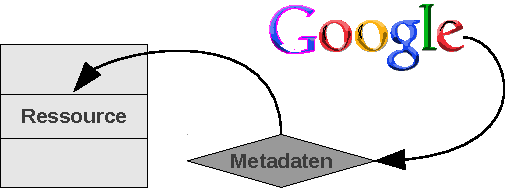
\includegraphics[scale=0.88]{images/metadaten_bild.pdf}}
		\caption{Funktion von Metadaten}
		\label{myfigure}
	\end{figure}
	
	\fbox{
		\begin{minipage}[t]{\columnwidth} 
			\vspace{3cm}
			Hier kommt noch eine Hinführung zu den Standards hin.
			\vspace{3cm}
			\hspace{\columnwidth}
		\end{minipage}
	}
	
	\section {Der Metadaten Standard MPEG-7 [A]} 
	
	\subsection {Einleitung}
	
	Der MPEG-7 Standard wurde 2002 von der \emph{Moving Picture Expert Group} als ISO/IEC 15938 verabschiedet. Im Gegensatz zu den früheren MPEG Standards (MPEG-1, MPEG-2 und MPEG-4) kein Kompressionsstandard für multimediale Daten sondern ein Metadaten Standard für selbige.
	
	Er bietet eine auf XML-Basierende umfangreiche Repräsentation von Metainformation für Audio- und Videodaten.
	
	Im folgenden wird der Standard im hinblick auf Audiosignale detailliert vorgestellt und seine automatisch generierbaren Aspekte vorgestellt.
	
	\subsection{Inhalt}
	
	Der MPEG-7 Standard spezifiziert vier Bestandteile:
	
	\begin{itemize}
		\item \emph{Descriptors}
		\item \emph{Descriptor Schemes}
		\item \emph{Description Definition Language}
		\item \emph{Binary Format für MPEG-7}
	\end{itemize}
	
	\subsubsection {Descriptors (D)}
	
Der erste Teil des Standards sind \emph{Descriptors}. Diese arbeiten auf räumlichen, zeitlichen oder physischen Segmenten der Ressource und  halten Daten zur Repräsentation eines Merkmals der Audiodatei.

	Dabei werden entweder gleiche Zeitintervalle der Ressource beschrieben oder sie wird in Segmente unterteilt und und Ähnlichkeiten und Differenzen werden aufgezeichnet. Beispiele für solche Descriptors sind der \emph{AudioWaveform} Descriptor welcher einem Intervall des Signals z.B. maximaler und minimaler Tonfrequenz zuweist.

	Diese Strukturen sind Low-Level und beinhalten lediglich die technischen Eigenschaften der Audio-Ressource. Es werden derzeit 17 \emph{Feature Descriptors} und ein spezieller \emph{Silence Descriptor} standardisiert. Diese 18 Strukturen sind in Untergruppen Organisiert (siehe Abb. 2).


\begin{figure}[h]
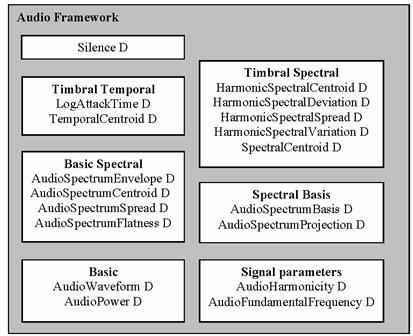
\includegraphics [scale=0.65]{image061.jpg}
\caption {Low-Level Descriptors in MPEG-7}
\end{figure}

Der \emph{Silence Descriptor} ist einfach die Darstellung das an dieser Stelle kein signifikanter Ton vorhanden ist und kann z.B. dazu eingesetzt werden ein Segment mit dieser Eigenschaft nicht weiter zu bearbeiten was die Erstellung der Metadaten effizienter macht.

	\subsubsection{Description Schemes (DS)}
		Der MPEG-7 Standard liefert neben den Low-Level Descriptors auch High-Level Description Tools in Form von \emph{Description Schemes}. Description Schemes beschreiben die Audiodatei auf einer höheren Abstraktionsebene und setzen dafür Descriptors und andere Description Schemes in Beziehung zueinander.
		
		Desciption Schemes nutzen die Rohdaten aus Descriptors und anderen Description Schemes um Audiodaten auf einem hohen Abstraktionsgrad zu beschreiben. Sodass Description Schemes die Struktur und die Semantik liefern in welcher die Descriptors und andere Description Schemes in Verbindung gesetzt wird. Damit kann man neben der rein technischen Low-Level Beschreibung der Ressource auch Charakteristiken wie Ton- , Instrumenten- und Melodie-Erkennung erzeugen und vermerken. 
				
	\subsubsection{Description Definition Language (DDL)}
Neben den bereits genannten Möglichkeiten bietet der MPEG-7 Standard ein weiteres mächtiges Werkzeug. Mit der Description Definition Language ist es möglich weitere, auf die Anforderungen des jeweiligen Nutzers zugeschnittene, Descriptors und Description Schemes zu entwickeln.

	Die Description Definition Language ist eine Erweiterung von XML-Schema.

\subsubsection{Binary Format für MPEG-7 BiM}

Das BiM ist entwickelt worden um die Metadaten schnell übertragen und streamen zu können. Das BiM bietet eine hohe Kompressionsrate der XML-Metadaten ( bis zu 98\%) und einen schnellen Zugriff auf Daten Entitäten im komprimierten Stream

\begin{figure}[h]
	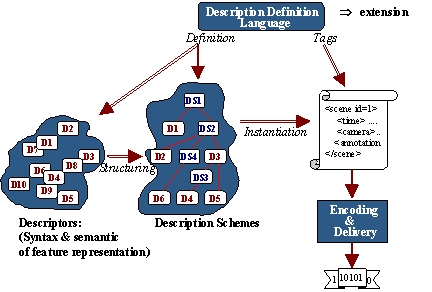
\includegraphics [scale=0.55]{image004.jpg}
	\caption {MPEG-7 Aufbau}
\end{figure}

	%\newpage
	\section{IPTC NewsML-G2 [B]}
	Im Jahr 2000 hat sich der Weltverband der Nachrichtenagenturen (International Press Telecommunications Council, IPTC) das Ziel gesetzt, technische Standards für den verbesserten Austausch von Nachrichten zu entwickeln und zu unterhalten. Damit soll der Austausch von Nachrichten, Sportinformationen und Angaben über Ereignisse auf internationaler Ebene verheinheitlich, vereinfacht und koordiniert werden.
	
	Um dieses Ziel zu erreichen hat der IPTC die Metadatenarchitektur \textbf{News Architecture G2} entwickelt, mit der der Austausch jeglicher Form von Nachrichten -- seinen es Bilder, Videos, Audioaufzeichnungen oder Texte in allen erdenklichen Formen auszutauschen. Dabei setzt der Verband auf ein Framework von drei Teilspezifikationen: EventML-G2 zur Beschreibung von Events, SportML-G2 für Sportveranstaltungen und NewsML-G2 zur Repräsentation und Verwaltung von Nachrichtenbeiträgen.
	
	Bei der Spezifikation wurde besonderes Augenmerk auf die Interoperabiltät zwischen Produzenten und Abnehmer, Erweiterbarkeit, Klarheit und einfache Speicherung gelegt. Zur Repräsentation wurde dafür das XML-Format gewählt.
	
	Die Architektur definiert dafür Blöcke (\enquote{building blocks}), welche mehrere Nachrichtenelemente (\enquote{news items}) enthalten können. Die Blöcke beschreiben die Art der Metadaten sowie Art und Struktur der (Nachrichten-)Elemente. Dabei können andere Elemente referenziert werden:
	
	\begin{figure}[htbp]
		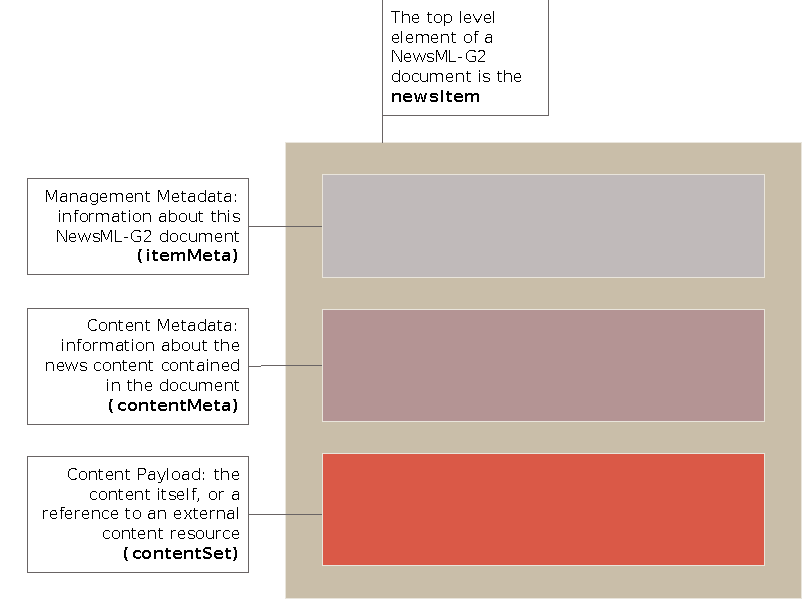
\includegraphics[width=\columnwidth]{images/iptc_news_item.pdf}
		\caption{Aufbau eines newsItems der NewsML-G2}
		\label{myfigure}
	\end{figure}

	Jedes newsItem muss dabei von einer eindeutigen ID gekennzeichnet sein sowie mit einer Versionsnummer.

	\begin{lstlisting}[caption=Beispiel-XML IPTC NewsML-G2 für die Europäische Hymne]{Name}
<newsItem xmlns="http://iptc.org/std/newsml/2006-10-01/"
   guid="urn:doi:cvce_audiovisual_4b6e5671-a0fc-45fa-8368-f84e4817dc14"
   version="1">
  <catalogRef />
  <itemMeta />
  <contentMeta />
  <contentSet>
    <remoteContent
      href="http://www.ena.lu/european_anthem-2-17815"
      size="8650645"
      contenttype="audio/wav"
      duration="134"
      audiobitrate="56"
      audiosamplerate="44100" />
  </contentSet>
</newsItem>
	\end{lstlisting}


	%\newpage
	\section{DER METADATEN STANDARD EBUCore [A]}
	
	\subsection{Einleitung}
	Der EBUCore ist ein Metadatenset welches von der \emph{European Broadcasting Union (EBU)} entwickelt wurde. Die EBU ist ein Zusammenschluss von 74 Rundfunkanstalten  in 56 Ländern Europas, Nordafrikas und Vorderasiens. Dieser Zusammenschluss produziert z.B. auch den Eurovision Song Contest.
	
	Der EBUCore ist eine Erweiterung des \emph{DublinCore}, welcher 1995 in Dublin/Ohio festgesetzt wurde. Der DublinCore spezifiziert eine Reihe von Metadaten zur beschreibung von Dokumenten im Internet.
	
	Im Jahr 2000 war es das anfängliche Ziel der EBU den DublinCore auf Audioarchive zu übertragen. Dieses Ziel wurde 2008 erweitert. Das neue Ziel war es den EBUCore so zu erweitern, das man mit den Metadaten nicht nur Daten im Archiv beschreiben kann, sondern mit ihrer Hilfe auch Archive durch z.B. Suchmaschinen im Browser durchsuchen kann.
	
	Die EBU sagt, dass heutige Ziele nicht mehr auf Audioressourcen und Archive beschränkt sind.
	
	Der bekanntesten Einsatzort des EBUCore ist derzeit die \emph{Europeana}. Die Europeana ist ein Projekt welches darauf abzielt, das kulturelle Erbe Europas zu digitalisieren und für jedermann zugänglich zu machen. Mithilfe des Webportals hat man Zugriff auf viele Millionen multimediale Ressourcen aus Europa und der Welt.
	
	Damit man diese Ressourcen auch nach der gewünschten durchsuchen kann, braucht es ein einheitliches Metadaten Format für Europa.
	
	\subsection{Der Standard}
	Der EBUCore ist eine minimale Liste von Attributen die man benötigt um eine multimediale Ressource zu beschreiben.Getreu dem Motto :\begin{quote}Wenn du's nicht findest, hast du's auch nicht.\end{quote} versucht die EBU durch den EBUCore einen allumfassenden Standard bereit zu stellen welcher eine Verbindung zwischen kulturellen Datenbanken, Produzenten multimedialer Ressourcen, Rundfunkanstalten, Archiven und Netzontologien herstellt.
	
	Auch der EBUCore nutzt das XML Format zur Repräsentation der Metainformation. Der Standard ist unter anderem in der EBU tech3293 spezifiziert.
	
	Anders als der MPEG-7 Standard muss der EBUCore komplett manuell erstellt werden. Dazu wird einfach ein XML-Instanz Dokument erstellt welches dem XML-Schema entsprechen muss.
	
	Das XML-Schema definiert über 30 Tags welche zur Beschreibung der Ressource dienen. Dabei werden neben den üblichen Beschreibungsformen, wie Titel oder Sprache, auch Tags angeboten die Informationen über das physikalische oder digitale  Format, Version oder Herausgabe Historie. Diese Tags spiegeln hier beispielhaft das bestreben produzierenden und konsumierende Gruppen unter einen Standard zusammen zu fassen.
	
	Es folgen nun zwei Beispiele wie ein XML-Instanz Dokument für ein Bild und eine Audioressource aussehen kann. Dabei kann man gut erkennen das der Standard komplett unabhängig von der zu beschreibenden Ressource fungiert.

\begin{lstlisting}[caption=Beispiel-XML EBUCore für Albrecht Dürers Bild: Adam und Eva]{Name}

<?xml version="1.0" encoding="UTF-8"?>
<schema xmlns:xsi=
"http://www.w3.org/2001/XMLSchema-instance" ...>

  <ebuCoreMain>
    <coreMetadataType>
      <title>Adam and Eve</title>
      <creator>Duerer, Albrecht (german painter) </creator>
      <description>...</description>
      <source>VADS</source>  
      <rights>The Bowes Museum Castle, Co. Durham</rights>
      <provider>CultureGrid; UK</provider>
      <subject>religion (Adam and Eve)</subject>
      <type>Physical Object</type>
    </coreMetadataType>
  </ebuCoreMain>
</schema>
\end{lstlisting}


\begin{lstlisting}[caption=Beispiel-XML EBUCore für die Europahymne]{Name}

<?xml version="1.0" encoding="UTF-8"?>
<schema xmlns:xsi=
"http://www.w3.org/2001/XMLSchema-instance" ...>

  <ebuCoreMain>
    <coreMetadataType>
      <title>Europahymne</title>
      <creator>van Beethoven, Ludwig</creator>
      <description>...</description>
      <source>
      	Dernier mouvement de la Neuvieme symphonie 
      	(Ode a la joie) ...
      </source>  
      <rights>
      	Centre Virtuel de la Connaissance sur l Europe (CVCE)
      </rights>
      <provider>ASSETS; Luxembourg</provider>
      <language>fr; en; de</language>
      <identifier>
      	doi_cvce_audiovisual_4b6e5671-a0fc-45fa-
      	8368-f84e4817dc14
      </identifier>
      <type>Physical Object</type>
    </coreMetadataType>
  </ebuCoreMain>
</schema>
\end{lstlisting}

Die beiden Beispiele sind sehr minimalistisch aber sie dienen dem Zweck einen großen Vorteil des EBUCore zu zeigen, die einfache Bedienung bei gleichzeitig relativ großer Beschreibungsmöglichkeit. Durch die weiteren Tags und zugehörige Attribute kann man von der Erstellung der Ressource (zum Beispiel mit dem Version-Tag) über die Auslieferung ( zum Beispiel Title oder Creator Tag)  bis zur Archivierung ( zum Beispiel das Subject Tag ).
\subsection{EBUCore und Semantic Web}

EBUCore liefert auch Bestandteile die für das Semantic Web genutzt werden können. Mit dem <realtion> -- Tag ist es möglich einzelne Ressourcen mit anderen in Verbindung zu setzen. Man kann aus verschiedenen Typen die gewünschte Relation ausdrücken. Beispiele hierfür sind : isPartOf, isRequiredBy oder isFormatOf.

	Ein weiterer Mechanismus der für das Semantic Web genutzt werden könnte, ist der <identifier> -- Tag. Mit diesem kann eine eindeutige Referenz auf die Ressource vermerkt werden, wie zum Beispiel ein DOI.
	%\newpage
	\section{DER METADATENSTANDARD TV-ANYTIME [A]}
	\subsection{Einleitung}
	Der TV-Anytime Standard ist vom TV-Anytime Forum spezifiziert worden. Das Forum setzt sich aus über 80 Mitgliedern aus Industrie und Unterhaltungsbranche zusammen. Die Ziele des Forums waren eine einheitlichen Standard für Audio-Visuelle Daten zu generieren, welcher dem Verbraucher eine bessere Übersicht über die Digitalen Programme liefern und auf ihn zugeschnittene Medieninhalte präsentieren soll.
	
	Der Standard soll in Systemen wie beispielsweise dem Personal Digital Recorder (PDR) Anwendung finden. Die Industrie ist daran Unterhaltungsindustrie ist daran interessiert damit der Verbraucher ihre Formate auch findet. Die Gerätehersteller wollen einen einheitlichen Standard um nicht für jedes System ein eigenes Gerät auf den Markt bringen zu müssen. Und letztlich der Verbraucher profitiert davon, da er Programme die ihn interessieren könnten präsentiert und eine strukturierte Übersicht über die Inhalte bekommt.

\subsection{Der Standard}
	Der TV-Anytime Standard ist so aufgebaut, das ein Nutzer mithilfe seines Gerätes schnell und einfach erfahren kann, welche Sendungen gerade angeboten werden, und welchen Inhalt diese haben. Dabei ist jedoch zu beachten,dass im Gegensatz zu den anderen Standards, hier auch ein werbender Charakter in die Beschreibung mit eingeht, damit der Nutzer auch von der Beschreibung zum Inhalt geführt wird.
	
	TV-Anytime nutzt XML-Schema Dateien, welche mithilfe der MPEG-7 Description Definition Language (DDL) erzeugt wurden.Diese definieren eine Dokumentenstruktur die sich aus verschiedenen Teilen zusammen wie zum Beispiel Informationen über:
	\begin{itemize}
		\item Programme
		\item Programmgruppen(z.B. Serien)
		\item Schauspieler
		\item und weitere
	\end{itemize}

	Damit ein Instanzdokument des Standards korrekt ist, muss man mindestens einen Programmtitel angeben, alle anderen Sektionen sind optional. Das TV-Anytime Forum empfiehlt jedoch zusätzlich noch mindestens die Zusammenfassung, das Genre, die Sprache und die Beteiligten Personen ( Schauspieler, Regisseur, Produzent etc.) mit anzugeben.
	
	Die Eben genannten Bestandteile fallen alle in das ProgramDescription Tag der XML Datei. Dieser beinhaltet auch noch Definitionen um Programme die mit dem aktuellen vergleichbar sind oder damit in Beziehung stehen zu vermerken, oder auch Trailer für die Ressource anzugeben.
 
 \subsection{Der Content Referencing Identifier (CRID)}
	Die Idee vom CRID ist das man in den Metadaten einer Ressource einen eindeutigen Verweis zur Ressource schafft. So kann man mit dem CRID über die Metadaten direkt zur Ressource gelangen. Auch hier war der Standard notwendig um eine einheitliche Identifikation der Ressourcen der verschiedenen Rundfunkanstalten und andere Inhaltslieferanten zu schaffen. Der CRID ist wie eine URL aufgebaut: \texttt{crid://<name>/<daten>}. \texttt{<name>} ist dabei wie ein DNS Name aufgebaut.

\subsection{Nutzerinformationen} 
	TV-Anytime spezifiziert Möglichkeiten um die Gewohnheiten der Nutzer hinsichtlich ihrer Programmauswahl zu speichern. Auch hier bedient der Standard sich der beiden Tags von MPEG-7 "user preference" und "usage history". Das Forum hat sich für auf ein einheitliches Modell zur Nutzerdatenspeicherung und Austauschen der Daten geeinigt.
	
	Das soll dazu dienen um dem Nutzer anhand seiner Gewohnheiten weitere Sendungen anzubieten die ihn interessieren könnten. Jedoch sollen diese Informationen auch dazu eingesetzt werden dem Nutzer personalisierte Werbung zu präsentieren.
	
	Mithilfe von Usage History und User Preferences wird es ermöglicht zu erfassen wie der Nutzer sich Inhalte anschaut, wann er Vorspult, auf Pause drückt oder etwas Aufnimmt. Mit diesen Informationen kann dann ein Nutzerprofil erstellt werden um das Angebot zu filtern, oder selbständig Inhalte aufzunehmen von denen der Recorder oder das zugrunde liegende System meint, es könnte den Nutzer interessieren.

	%\newpage
	\section{Vergleich [A, B]}
	\subsection{Nutzer}
	Die verschiedenen Standards haben auch verschiedene Nutzer. Der \textbf{MPEG-7} Standard wird vorrangig von Algorithmen zur Suche verwendet um zum Beispiel \enquote{Query By Humming} Anfragen zu bearbeiten. Das liegt auch daran dass fertige MPEG-7 XML Dateien durch die vielen Descriptors welche beispielsweise im 10 ms Intervall eine Audioressource abtasten.
	
	Der \textbf{EBUCore} kann durch seine einfache Bedienung und seine dennoch große Vielfalt von jedem eingesetzt werden. Derzeit ist der größte Nutzer die Europeana und die angeschlossenen Projekte wie: ECLAP, Digital Contemporary Art, EUScreen und andere.
	
	\textbf{NewsML-G2} ist ein Standard der nur von Nachrichtenagenturen eingestzt wird. Er ist weltweit im Einsatz und dient zur kommunikation zwischen den Agenturen.
	
	\textbf{TV-Anytime} wird vom Endverbraucher genutzt. Er kann über TV-Anytime Informaionen zur Ressource erhalten und auch selber Informationen wie zum Beispiel Meinungen eintragen.

	\subsection{Abstraktionsgrad}
Der Abstraktionsgrad der Standards unterscheidet sich stark. \textbf{MPEG-7} hat einen sehr hohen Abstraktionsgrad. Er bietet die Möglichkeit die Audioressource über die physikalischen Eigenschaften hinaus auf ein hohes Niveau bis zur Notenerkennung und Automatischer Spracherkennung ( Automatic Speech Recognition, ASR).\textbf{TV-Anytime} ist ebenfalls auf einem hohen Level der Abstraktion. Es bietet neben der Beschreibung von Inhalten, Regie und Mitwirkende auch die Möglichkeit Bewertungen von Benutzern über den Inhalt einzusehen und so auch eine Kommunikation statt eine reine Distribution zu gewährleisten.

	Dagegen sind die beiden anderen Spezifikationen eher auf einer geringen Stufe der Abstraktion. \textbf{EBUCore} und \textbf{NewsML-G2} bieten lediglich eine Beschreibung der Ressource auf allgemeiner Ebene wie Inhalt und beteiligte Personen. Dies ist jedoch keinerlei Nachteil, da sie genau dafür entwickelt wurden.

	\subsection{Generierung}
	Man kann die Standards hinsichtlich der Generierung in zwei Gruppen teilen. Die eine Gruppe bildet der \textbf{MPEG-7} Standard welcher mithilfe von Applikationen und Werkzeugen nahezu automatisch generiert werden kann.
	
	Die andere Gruppe sind \textbf{EBUCore}, \textbf{TV-Anytime} und \textbf{NewsML-G2}. Diese lassen sich nicht automatisch generieren sonder werden manuell erzeugt.

	\subsection{Stelle in der Verwertungskette}
	\textbf{MPEG-7} befindet sich im hinteren Teil der Verwertungskette. Durch die Anwendung von Algorithmen kann ein Benutzer direkt mit den MPEG-7-Daten interagieren. %TODO
	
	\textbf{NewsML-G2} wird nach der Produktion eines Nachrichtenbeitrags zur Archivierung und Verarbeitung innerhalb der Nachrichtenagenturen eingesetzt. Dieser recht eng gefasste Einsatzrahmen wird kaum verlassen.
	
	Das \textbf{EBUCore}-Metadaten-Set findet Anwendung über die gesamte Verwertungskette, von der Produktion über Austausch mit anderen Parteien bis zur Archivierung.
	
	\textbf{TV-Anytime} findet seinen Einsatz hauptächlich beim Endanwender, beispielsweise in Set-Top-Boxen für den TV-/Radioempfang. Der Dienstanbieter (etwa der Rundfunksender) bereitet die Daten hierfür entweder händisch oder aus anderen Metadaten auf.

	\subsection{Zweck}
	Einer der Hauptanwendungszwecke von \textbf{MPEG-7} ist die intuitive Suche per Eingabe in natürlicher Sprache. Die MPEG stellt jedoch explizit fest, dass der Standard nicht auf einen spezielle Anwendung abziehlt. Zusammenfassend wird MPEG-7 jedoch fast ausschließlich von Algorithmen und Computern genutzt.

	\textbf{NewsML-G2} wurde für den einfachen Austausch von Nachrichten innerhalb von Agenturen -- auch über Länder- und kulturelle Grenzen hinweg -- entwickelt. 
	
	Das ursprüngliche Ziel von \textbf{EBUCore} war die Übertragung des Dublin-Core-Sets von (Web-)Dokumenten auf multimediale Ressourcen. Später sollte ein gemeinsamer Kern an Metadaten für Archive entstehen; heute wird der Standard hauptsächlich für multinationale Großprojekte auf EU-Ebene genutzt. 
	
	\textbf{TV-Anytime} soll die Fragmentierung herstellerspezifischer Metdaten für Empfangsgeräte homogenisieren. 
	
	%\newpage
	\section{Verhältnis zwischen XML und RDF/OWL (Semantic Web) und SKOS für classification schemes [B]}
	\subsection{RDF, RDFS und RDF/XML}
	\subsubsection{RDF}
	Das Resource Description Framework (RDF) ist eine universelle formale Sprache zur Beschreibung von strukturierten Informationen (ursprünglich: Metadaten im Web). Mittels RDF werden Information über so genannte Ressourcen gespeichert. Ressourcen sind Uniform Ressource Identifiers (URIs), die eine Quelle referenzieren. Diese Ressourcen können Webseiten, ISBNs für Bücher und Zeitschriften oder DOIs (zum Beispiel doi:10.1000/182) sein.
	
	Metadaten werden als Tripel -- Subjekt, Prädikat, Objekt -- gespeichert. Dabei wird die Beziehung zwischen Subjekt und Objekt angegeben. Die Beziehung \enquote{\enquote{Die Glocke} ist von Friedrich Schiller geschrieben} ergibt das Tripel \enquote{Die Glocke} (Subjekt), \enquote{ist geschrieben von} (Prädikat), \enquote{Friedrich Schiller} (Objekt). Zur Notation nutzt man häufig die (inoffizielle) \emph{Turtle}-Syntax. % Obiges Trippel sieht in dann so aus: % TODO: evtl. Turtle-Syntax
	Auf diese soll hier jedoch nicht eingegangen werden, da in der Praxis überwiegend die Serialisierung mittels Extensible Markup Language (XML) genutzt wird.
	
	\subsubsection{RDF/XML}
	Dieses vom W3C standardisierte Format wird RDF/XML gennant. \prettyref{lis:rdfxml} zeigt ein Beispiel für obige Beziehung in RDF/XML. Dabei wurden zusätzlich einige Elemente der Dublin-Core-Spezifikation genutzt.
	% TODO: placement on the same page!
	%\lstinputlisting[float=*b, language=XML, caption=Beispiel für XML/RDF, label=lis:rdfxml]{files/schiller.rdf}

	\subsubsection{RDFS}
	RDF benötigen zur \emph{Interpretation} der dargestellten Beziehungen ein gemeinsames Vokabular, zum Beispiel Dublin Core. RDF Schema (RDFS) stellen dafür ein Vokabular zur Verfügung, mit dessen Hilfe innerhalb von RDFS-Dokumenten Aussagen über semantische Beziehungen der Termini gemacht werden können. Es handelt sich dabei nicht um ein thematisches Vokabular; vielmehr 

	\subsection{OWL}
	Web Ontology Language (OWL) ist eine Spezifikation des W3C, die entwickelt wurde, um...
	
	OWL basiert auf RDF/XML, fügt jedoch weitere Ausdrücke zur Beschreibung von Eigenschaften und Klassen hinzu. Damit werden Aussagen ähnlich der Prädikatenlogik ermöglicht (Disjunktheit, Aussage "genau einer", Äquivalenz...)
	
	OWL bietet drei Untersprachen mit steigender Ausdrucksstärke (\emph{OWL Lite}, \emph{DL} (description logic) und \emph{Full}) und unterschiedlichen Zielgruppen. OWL Lite ist eine (echte) Teilsprache von OWL DL, welches wiederrum eine (echte) Teilsprache von OWL Full ist.
	
	% http://www.semaweb.org/dokumente/w3/TR/2004/REC-owl-features-20040210-DE.html, 28.05.2011, 13:13
	% Hitzler, Pascal, et. al. Semantic Web,	Berlin [u.a.] Springer, 2008, Seite 127
	
	\subsubsection{OWL 2}
	% TODO
	
	\subsection{SKOS}
	Simple Knowledge Organization System (SKOS) ist eine vom W3C spezifierte formale Sprache zum Verteilen und Verlinken von Informationsystemen wie Thesauri, Taxonomien und Normdateien im Web. SKOS basiert auf RDF und RDFS.
	% http://www.w3.org/TR/skos-reference/, 28.05.2011, 15:27
	
	SKOS soll die Nutzung von concept schemes im Web im Vergleich zu OWL erleichtern. OWL verfolgt das Ziel, komplexe Konzeptstrukturen auszudrücken, um so ausführliche Metadaten zu generieren und Schlussfolgerungswerkzeuge zu unterstützen. Die Erstellung sinnvoller Web-Ontologien ist jedoch sehr aufwändig, und in vielen Fällen werden die zahlreichen Möglichkeiten der OWL nicht benötigt. Deshalb kann hier der Einsatz von SKOS vorteilhaft sein.

	% http://en.wikipedia.org/wiki/Simple_Knowledge_Organization_System vom 13:30, 12 May 2011. 28. Mai 2011, 15:37

	\section{Media Annotations Working Group [B]}
	Dieser Überblick zeigt, dass es verschiedene Metadaten-Standards für Audio-, Video und Bildsignale gibt, die unterschiedliche Zielstellungen, Herangehensweisen und Lösungsansätze bieten. Allerdings gibt es auch größere Schnittmengen zwischen den Standards, und für vollständige (semantische) Angaben kann es nötig sein, Elemente aus verschiedenen Metadaten-Sets zu nutzen.
	
	Aus diesem Grund hat das W3C eine Arbeitsgruppe gegründet, die sich mit der Zusammenführung genannter Standards (und weiteren) befasst. Die \emph{Media Annotations Working Group (MAWG)} hat sich zum Ziel gesetzt, die Interoperabilität zwischen Metadaten-Standards für Multimediaressourcen zu verbessern.
	
	Dazu hat die Gruppe eine Menge von Standards identifiziert, die untereinander kompatibel sein sollen. Dazu gehören neben den hier genannten Dublin- und EBUCore, IPTC % TODO: did we?
	sowie MPEG-7 zum Beispiel auch der für Fotos genutzte EXIF-Satz sowie anbieterspezifische Metadaten wie die von Youtube, Apple und Adobe. Eine vollständige Übersicht unterstützer Standards bietet [X]. %http://www.w3.org/2008/WebVideo/Annotations/drafts/ontology10/CR/mappings_tested/ % TODO!
	
	Um dieses Ziel zu erreichen hat die Arbeitsgrupppe eine \enquote{Media-Ontologie} geschrieben, in welche sowohl semantische als auch syntaktische Abbildungen der wichtigsten Elemente aus den einzelnen Metadaten-Spezifikationen existieren sollen. Ein vollständiges Mapping aller Elemente wird dabei ausdrücklich nicht angestrebt.
	% http://mawg.joanneum.at/web/mawg.html#mission, 28. Juli 2011, 9:28
	% http://www.w3.org/2008/01/media-annotations-wg.html#scope, 28. Juli 2011, 9:43
	
	Mit dieser Ontologie soll es beispielsweise möglich sein, ID3-Tags %TODO
	
	Diese \emph{lingua franca} der Metadaten soll auserdem eine Programmierschnittstelle (Applikation Programming Interface, API) bieten, um die extrahierten Informationen leicht abrufen zu können. Dabei soll in einer ersten Iteration zumindest der lesende Zugriff über JavaScript ermöglicht werden; weitere Versionen werden zusätzlich (schreibenden) Zugriff mittels JavaScript und einem einfachen RDF-Format bieten.
	
	\bibliographystyle{phcpc}
	\bibliography{references}
\end{document}